\documentclass[../main/main.tex]{subfiles}


\begin{document}
\section{How life generates order}

\newdate{date}{03}{03}{2023}

\marginpar{ \textbf{Lecture 2.} \\  \displaydate{date}. \\ Compiled:  \today.}

Biological machines are then completely different from traditional macroscopic ones. The thermodynamic paradigm of living systems is to seek for an interface of an energy flux and to take advantage of order (input), to degradate this order into disorder and, in this process, being able to control and organize the entropy of the organism. 
To give a practical example, we can consider the bio-chimical reactions that happen in plants thanks to which they are able to store part of the energy coming from the sun, so high quality energy $\Delta U>0$ carried by photons hitting the the surface perpendicularly, and then to convert it into chemical energy that can later be used to fuel the organism's activities. 
In this process - \emph{cellular respiration process} - the energy is employed to preserve or diminisch the entropy of the organism itself and part of this energy is released in the environment as a form of low quality energy in any directions.

\begin{wrapfigure}{r}{0.35\textwidth}
    \centering
    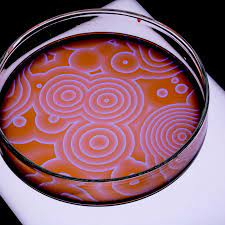
\includegraphics[width=0.8\linewidth]{../frontespizio/tikz/1_lesson/Belousov-Zhabotinsky reaction.jpeg}
    \caption{B.-Z. reaction\cite{nat_geo}.}
\end{wrapfigure}

Another example can be the Belousov-Zhabotinsky reaction: what we observe is the formation of structures, patterns, as over time we can think of this as an increase in order and consequently a dicrease in disorder of the system. The energy flux coming from the reagents of the reaction leaves behind an increase of order and when there is no more external energy the system slowly comes back to its original disordered state, and patterns can not been seen. 
By taking advantage of order - input energy - and degradating this order into disorder, living systems are so able to control and organize the entropy of the organism the death can be pictured as the maximum possible entropy state a system can reach. When there is no longer the possibility to control this order-disorder mechanism a system is considered dead.

\subsection{A paradigm for free energy transduction: osmosis flow}
A cylinder filled with water is separated into two chambers by a semipermeable membrane which is anchored to the cylinder \cite{biological_physics}. Two pistons slide freely allowing the volumes of the two chambers to change as water molecules cross the membrane. Since the water is incompressible, the two pistons must slide together. The open white circles in the picture are sugar molecules and they are confined in the right-hand chamber. 
As long as the weight is not too heavy \textbf{(a)} when the pistons are released we observe an osmotic flow as water crosses the membrane, forcing the both pistons to the right and lifting the weight. The sugar molecules then spread out into the increased volume of water on the right. 
As the sugar dissolves and spreads through the right-hand chamber, a mysterious force begins to push the pistons to the right: the energy needed to lift the weight came from the outside world, as the system absorbs heat from its surroundings and somehow this thermal energy is converted to mechanicl work. But, it is impossible to completely convert heat into mechanical work, so the order of the sugar molecule is used up: initially each one moves freely, and randomly, throughout the region
between the membrane and the right-hand piston. 

\begin{figure}[h!]
    \centering
    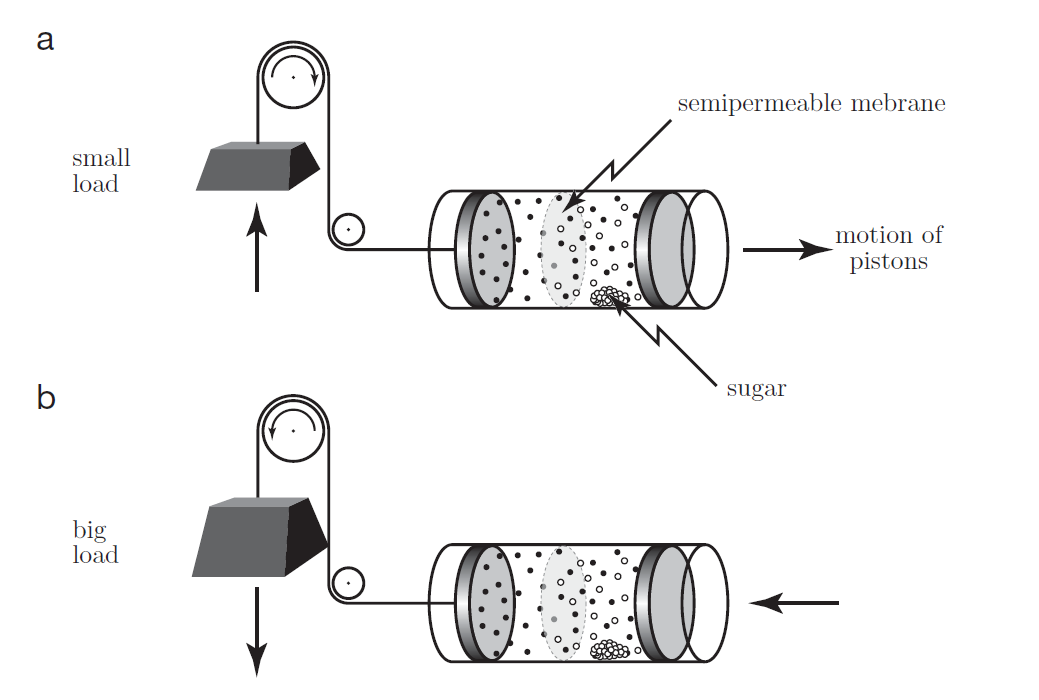
\includegraphics[width=0.6\textwidth]{../frontespizio/tikz/1_lesson/osmosis.PNG}
    \caption{A mechanical mechanism trasducting free energy.}
\end{figure}

As water flows through the membrane, forcing the pistons to the right, the sugar molecules lose some of their order (or gain some disorder), being no longer confined to just one half of the total volume of water. When finally the left side has shrunk to zero, the sugar molecules have free run of the entire volume of water between the pistons; their disorder can't increase any more. Osmotic flow sacrifices molecular
order, to organize random thermal motion into gross mechanical motion against a load. This can be summarized into the two conditions that must be satisfied $\Delta U>0 $ (the potential energy of the weight increases) and $\Delta S>0$ (decrease in order), since in the end $\Delta F \leq 0$ as stated by the $2^{nd}$ principle. \\
On the contrary, the reverse ormosis can be seen in \textbf{(b)} where if the weight is pulled hard enough downward, the pistons will move to the left increasing the concentration of the sugar solution in the right-hand chamber, generating heat. In this case, $\Delta U<0$ as well as $\Delta S<0$ such that $\Delta F <0\implies \frac{\Delta U}{T} < \Delta S$. This is the perfect example we were looking for: an external input energy - mechanical work in this case - improves the order of our system ($\Delta S <0$). 
In agreement with the $1^{st}$ principle, the energy input must go somewhere and in fact the system gives off heat in the process, to the outside world.\\
Reverse osmosis is similar to what happens into chloroplasts and plants, where mechanical energy is provided by photons, and the result is the production of order by the production of ATP or more sophisticated molecules. In the same manner, animals too use chemical energy, rather than mechanical or light one, to keep themself organized, by ingesting food rich of bio-chemical compounds.


\section{Density, current and flux}
Doing physics experiments on anthropic scale, we are familiar with common units such as \emph{meters}, \emph{kilos}, \emph{liters} and so on... but, what are the units and the abstract dimensions of things in the biological physics realm? 
We will say, for instance, that \emph{length} has dimensions $\mathbb{L}$, so writing $[L] = \mathbb{L}$, measured in meters $m$ in \textbf{SI} units. We point out that dimensions are distinct from units so, considering more examples, \emph{mass} has dimension $\mathbb{M}$ expressed in $kg$ in SI units; \emph{time} has dimension $\mathbb{T}$ measured in seconds $s$ in SI units; \emph{energy} has dimension $\mathbb{ML^2T^{-2}}$ expressed in joules $J$ in SI units. \\ 
These are just some examples useful to explain very important relations between units: recalling that a \emph{liter} is equal to a cubic decimiter we can write that $\frac{1L}{1dm^3}\equiv1$ and so, using also $\frac{1m}{10dm}\equiv1$ we can perform a unite conversion, such as $1L\cdot 1 = 1L\cdot\frac{1dm^3}{1L}\cdot(\frac{1m}{10dm})^3 = 10^{-3}m^3$.

We can consider an additive and trasportable quantity $\mathcal{Q}$, such as linear momentum, energy, or the electric charge or even the number of particles in our system, and given the three dimensional space $\mathcal{V}$, we are able to compute the volume in which this quantity live: $V=\int_{\mathcal{V}}dV$. From this definition we can express other useful physical quantities such as the density $\rho_{\mathcal{Q}}(\vec{r}, t)$ (a field quantity), thanks to which we are able to find $\mathcal{Q}(t)=\int_{\mathcal{V}}dV\rho_{\mathcal{Q}}(\vec{r}, t)$, where
$[\rho_{\mathcal{Q}}]=\frac{[\mathcal{Q}]}{\mathbb{L}^3}$. Keeping $\mathcal{Q}$ the more generic as possible we are able to distinguish between charge density $\rho_c$ and mass density $\rho_m$ (?).
As well as volumes, we can define areas as $A=\int_{\mathcal{A}}dA$ where $\mathcal{A}$ represents the oriented surface, and from this definition we can finally define the net amount of $\mathcal{Q}$ passing through $\mathcal{A}$ per unit time, so the current $I_{\mathcal{Q}}(t)=\int_{\mathcal{A}}\vec{J}_{\mathcal{Q}}(\vec{r},t)\cdot d\vec{A}$ where $\vec{J}_{\mathcal{Q}}(\vec{r},t)$ is the flux - or current density - of particles. Pay attention that since $[A_{\mathcal{Q}}]=\frac{[\mathcal{Q}]}{\mathbb{L^2 T}}$, then $[I_{\mathcal{Q}}]=\frac{[\mathcal{Q}]}{\mathbb{T}}$.

Within $\mathcal{V}$ there could be also the production $\Pi_{\mathcal{Q}}(t)$ of a certain amount of $\mathcal{Q}$ per unit time. The volumetric production rate is indicated with $\pi_{\mathcal{Q}}(\vec{r},t)$ and it is another field quantity. Then $\Pi_{\mathcal{Q}}(t) = \int_{\mathcal{V}}dV\pi_{\mathcal{Q}}(\vec{r},t)$. In this manner we can define the \emph{integral balance equation} as $$\frac{d}{dt}\mathcal{Q}=-I_{\mathcal{Q}}(t)+\Pi_{\mathcal{Q}}(t)$$ and using Gauss theorem we can pass to the \emph{differential form}: 
\begin{equation}
    \frac{\partial}{\partial t}\rho_{\mathcal{Q}}(\vec{r},t)=-\vec{\nabla}\cdot\vec{J}_{\mathcal{Q}}(\vec{r},t)+\pi_{\mathcal{Q}}(\vec{r},t)
\end{equation}
which is known also as \textbf{continuity or balance equation}\footnote{All the $\vec{r}$ coordinates are \emph{eulerian}, but later on in the course we will consider \emph{lagrangian} coordinates and we will introduce total (or material) derivatives.}. This equation is fundamental because it expresses how the density is related with the flux of the quantity we are considering and reminds us of the continuity equation in electromagnetism\footnote{\href{https://en.wikipedia.org/wiki/Continuity_equation\#Differential_form}{Continuity equation in electromagnetic theory}}. 

\subsection{Negligibility of quantum effects}
Consider this simple problem: \emph{Given $N_{mol} = 6.0\cdot10^{23}$ the number of Avogadro, estimate the size of a water molecule}. 

\begin{wrapfigure}{l}{0.5\textwidth}
    \centering
    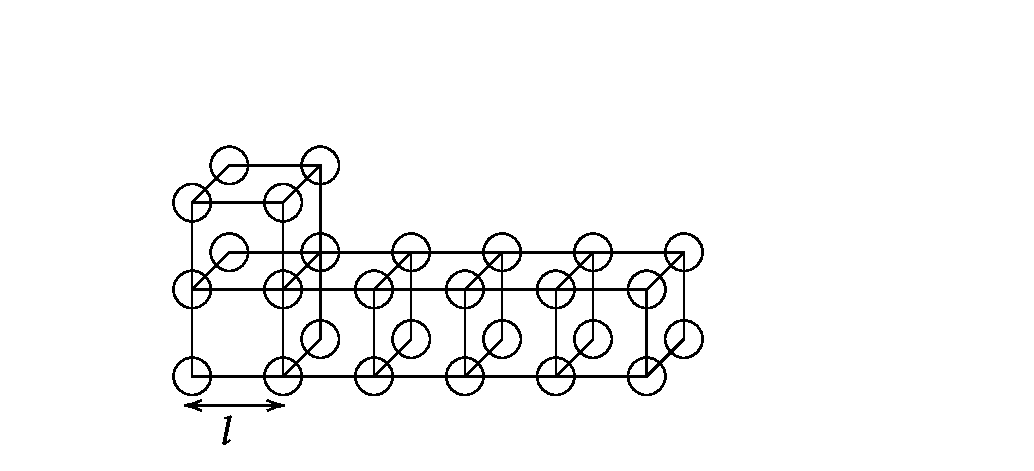
\includegraphics[width=0.6\textwidth]{../frontespizio/tikz/1_lesson/exercise.pdf}
    \caption{\label{fig:water} Cubic lattice of a water molecule.}
\end{wrapfigure}

To solve this problem recall that $\rho_{m, H_2O}=1kg/L = \frac{m_N}{V}=\frac{m_N}{NV_c}$. Supposing we are dealing with a cubic lattice of size $l$, so that each particle has its own cube, except for those at the surface, and supposing we are considering a great size of particles so that we can state that surface effects are negligible with respect to bulk effects, in this way $V_c = l^3=\frac{m_N}{V}=\frac{m_N}{V\rho_{m, H_2 O}}=\frac{\underbrace{n\cdot MM_{H_2 O}}_{18g/mol}}{N\rho_{m,H_2 O}}=\frac{18g/\cancel{mol}}{6.0\cdot10^{23}\cancel{mol^{-1}}\cdot\frac{1kg}{L}}=30\cdot10^{-30}m^3$ so, in other words, the size of a water molecule is $l=3.1\cdot 10^{-10}\:m=0.31\:nm$. 
This result doesn't only show the dimensions of a water molecule and the effectiveness of dimensional analysis, but also allows us to neglect quantum effect, since we will generally work always above this threshold.

\begin{figure}[h!]
    \centering
    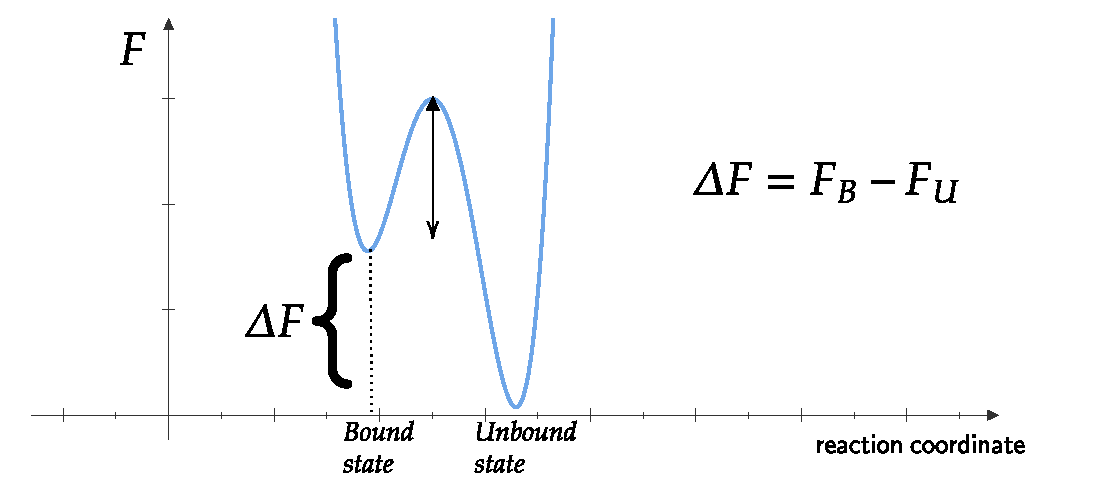
\includegraphics[width=0.7\textwidth]{../frontespizio/tikz/1_lesson/free_energy.pdf}
    \caption{Possible free energy landscape of a molecule.}
\end{figure}

As before mentioned, reactions flows in order to decrease the the value of the free energy $F$, but to stop biological processes and to keep molecules into \emph{bound states}, enzymes are employed: they play a key role in biological processes since they are able to increase or decrease the activation energy barrier allowing some reactions to happen faster and preventing others to occur\footnote{By \emph{allosteric control} in biochemistry we refer to the regulation of conformational change in protein dynamics of an enzyme.}.
Typical $\Delta F$ of chemical bonds are of the order of $\Delta F=q|\Delta V|=2.4\cdot10^{-19}\:J=240\:pN\cdot nm$, having considered a $\Delta V=1.5\:V$ and the electric charge $q$ of an electron. The free energy has been expressed both in $J$ and $pN\cdot nm$ to underline the order of magnitude of the quantities involved. We are therefore considering forces that act on the picoNewton scale (trillion times smaller than those we are used to on an anthropic scale) and nanometer distances.
Pheraps the most important formula to remember is the \textbf{thermal free energy} $\Delta F_{ther}=k_B T_r=4.1\cdot10^{-21}\:J=4.1\:pN\cdot nm$ which represents the thermal energy of the \emph{reservoir}, so the thermal bath surrounding the system under study. We can see that there is a consistent difference between the thermal free energy and the typical one before mentioned, meaning that we need thermal activation energy for processes to occur, but it is also fundamental to have stable chemical bonds.  

\subsection{Equipartition theorem}
Last but not least key element of this introduction on biological physics is the equipartition theorem which states that, at thermal equilibrium, energy is shared equally among all of its possible forms. Traslated into physics, this means that each quadratic-term of the hamiltonian of the system contributes with a $1/2 k_B T$ factor to the average kinetic energy in thermal equilibrium. 
This means that from the mean kinetic energy $\vmedvec{\frac{1}{2}m\vec{v}^{\:2}}=\frac{1}{2}m\vmedvec{\underbrace{\vec{v}^{\:2}}_{v_x^2+v_y^2+v_z^2}}=\frac{3}{2}k_B T\implies \sqrt{\vmedvec{\vec{v}^{\:2}}}=\sqrt{3\frac{k_B T}{m}}\simeq 640\:m/s$, $T$ being the room temperature. This last result is of great importance too since expresses the average velocity of water molecules. 

\chapter{Molecules are small, but how much?! A journey inside living cells}

\begin{chapquote}{Italo Svevo}
    La vita non è né brutta né bella. È originale.
\end{chapquote}

We are now ready to look a bit closer to the organization of the cells, where same ideas are used and used in many different ways.  The goal of this chapter is just to give an idea fo the spatial scales of different organism that we will study in future chapters and to give an insight on the hierarchy of scales in cells. By looking at different size devices, we will try to answer the following question: \emph{how can cells keep track of everything?}  
\begin{figure}[h!]
    \centering
    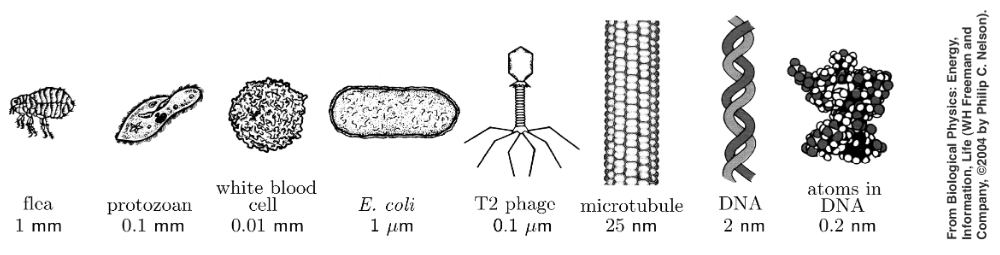
\includegraphics[width=0.95\textwidth]{../frontespizio/tikz/1_lesson/spatial_scales.PNG}
    \caption{Relative sizes of some of the protagonists of this chapter.}    
\end{figure}
The above picture shows many peculiar biological actors: starting from a common flea, we are capable to see up to the \emph{Escherichia coli}, which is quite invisible to the naked eye, since the the human eye's resolution limit is of order of $100\: mu m$ (\emph{in-vivo}). We know that the objects above pictured have that shape thanks to lenses and visual light employed in electron microscopy (\emph{in-vitro}), which has a resolution limit of ~$0.1\:nm$.

\begin{figure}[h!] 
    \centering
    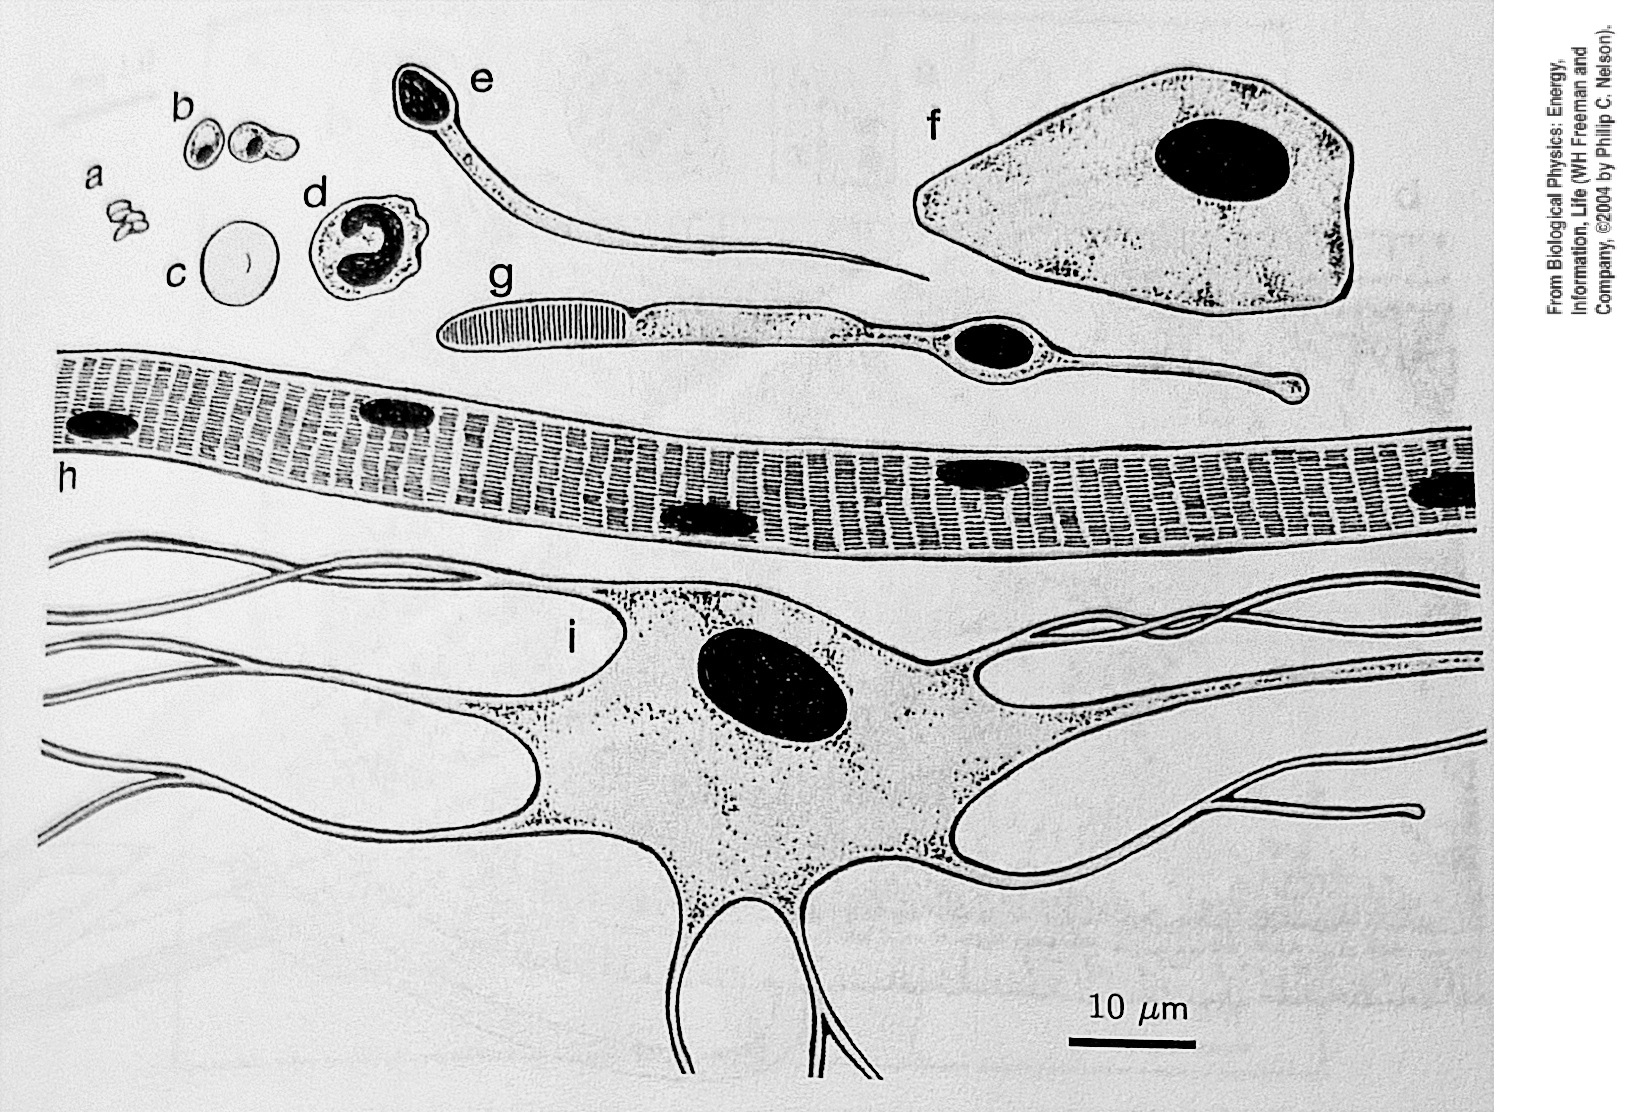
\includegraphics[width=0.49\textwidth]{../frontespizio/tikz/1_lesson/Drawing.jpg}
    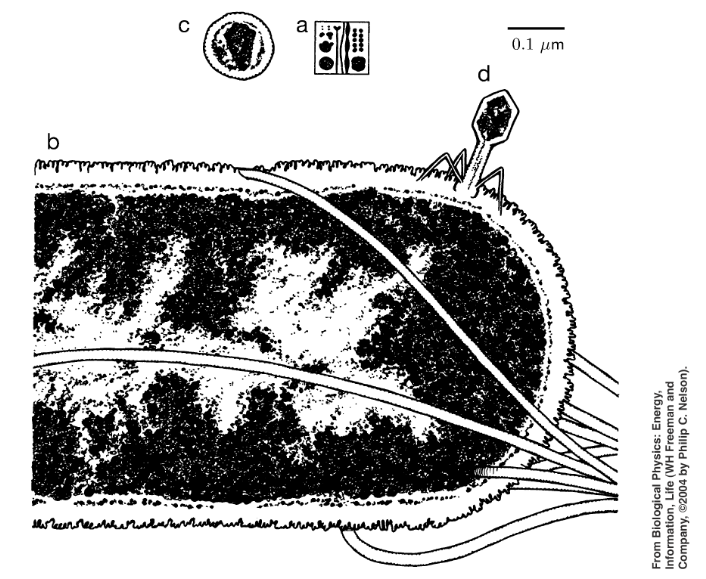
\includegraphics[width=0.49\textwidth]{../frontespizio/tikz/1_lesson/drawing_electron.PNG}
    \caption{\label{fig:2_2} Drawing based on light and electron microscopy: relative sizes.} 
\end{figure}

Setting the scale at $10\mu m$ we can compare (Figure [\ref{fig:2_2}]) the dimensions of \emph{Escherichia coli} bacteria cells (a) with two cells of baker's yeast (b), whihc are smaller than a human red blood cell (c). Human white blood cell (d) are instead a little bit bigger, but not as much as a human sperm cell (e), or a human skin (\emph{epidermal}) cell (f). On this scale, human photoreptor cells (g), human striared muscle (\emph{myocyte}) cells (i) and also a typical human (\emph{neuron}) nerve cell (i) are the biggest sized actors. Zooming in, on a $0.1\mu m$ scale, we can spot several (a) molecules and macromolecules (such as glucose and ATP molecules, t-RNA, antibodies, DNA and generic enzymes) in comparison with a bacterial cell (b) with its peculiar structure made of flagella, nucleotides and a rigid cell wall. It's easy to distinguish (d) a bacterial virus which has the same dimension of the human immunodeficiency virus (c). 
In the same cartoon extremely different cells are juxtaposed, thinking of neurons capable of receving and outputting electrical signals or bacteria able to live in extreme environmental conditions\footnote{In recent years, a number of studies have claimed that ancient bacterial cells are able to survive at very high temperature and to repair their DNA, thanks to an high stress tolerance and resistance to adverse conditions\cite{bacteria}}, or further viruses which have a parassitic or symbiotic relationship with the hos. But, they still share similiraties such as the way these micro-elements keep themselves organized by using \emph{active transport}, for example, to bring syntesized materials to particular destinations or biochemical reactions to compute highly specific processes.   

\end{document}
